\begin{frame}{Giao diện - Xác minh mã xác thực hai lớp (MFA)}
\begin{figure}[H]
\centering
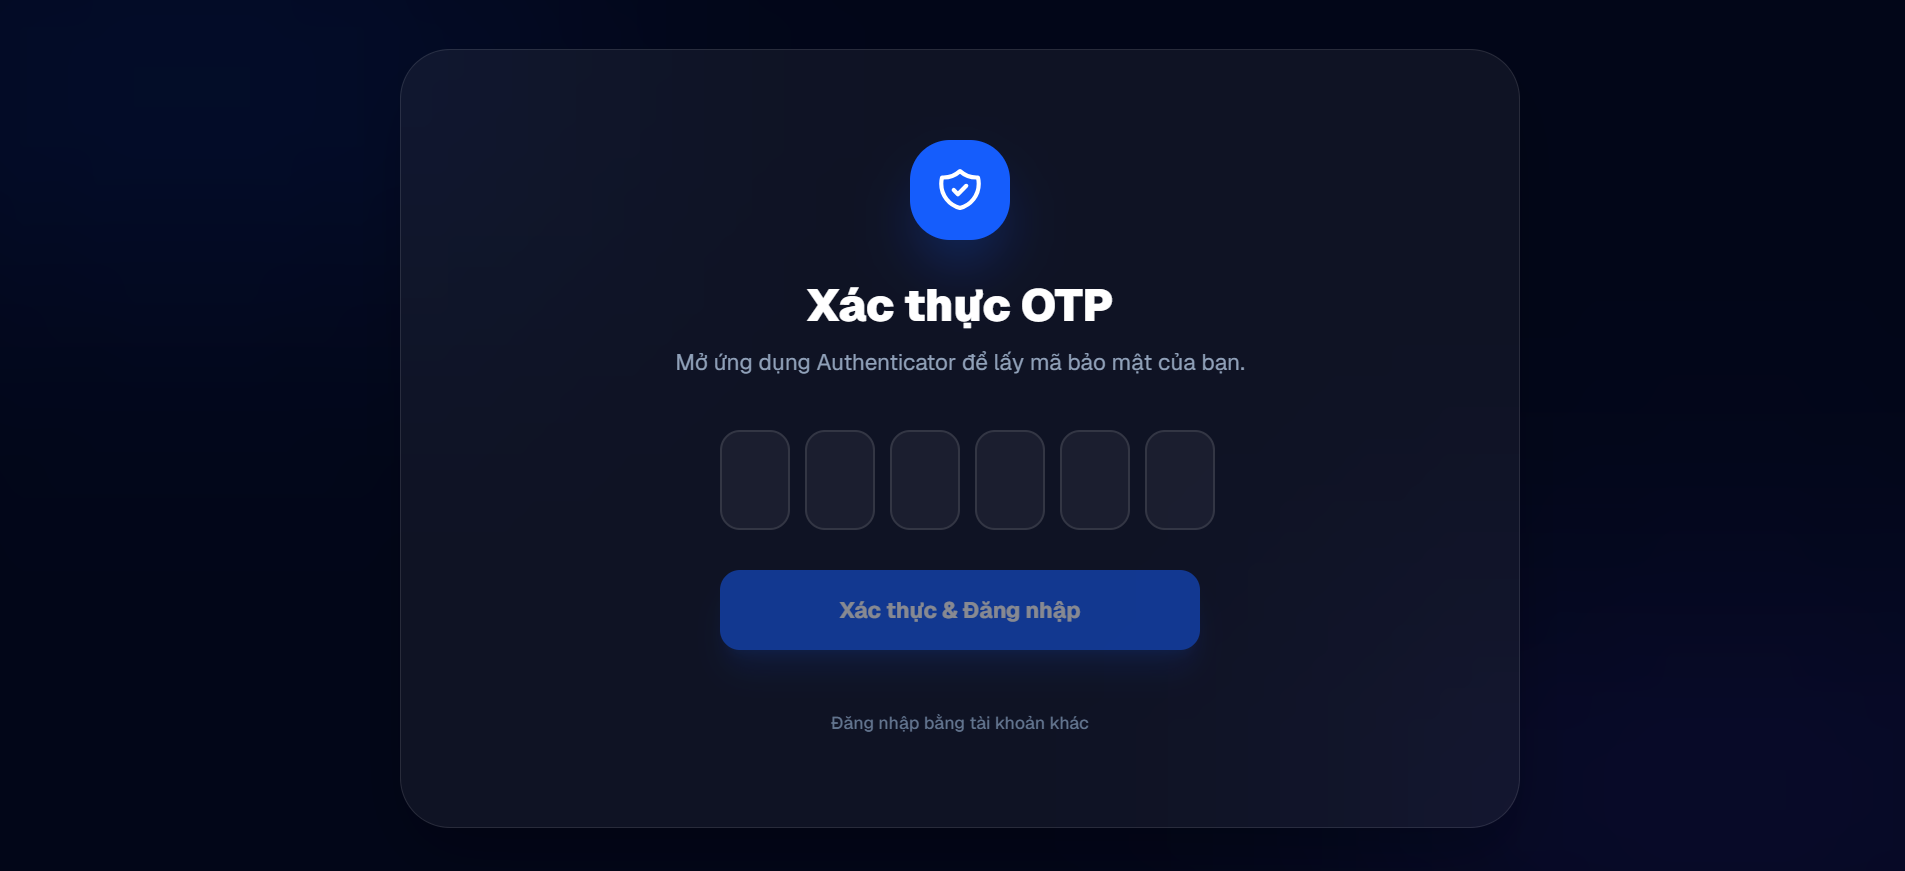
\includegraphics[height=0.55\textheight,width=0.9\textwidth,keepaspectratio]{pictures/WebUI/WebUI-MfaCodeVerify.png}
\caption{Giao diện xác minh mã MFA}
\end{figure}

\note{
Sau khi quét mã QR thành công, người dùng tiến hành bước xác minh mã để kích hoạt hoàn toàn tính năng MFA.
Người dùng nhập mã số gồm 6 chữ số đang hiển thị trên ứng dụng Authenticator vào ô xác minh trên giao diện. Hệ thống sẽ gọi API của Supabase để kiểm tra tính hợp lệ của mã số này. Nếu chính xác, trạng thái bảo mật của tài khoản sẽ được nâng cấp lên mức cao hơn (aal2) và tính năng MFA được kích hoạt chính thức.
}
\end{frame}
